% третья часть

\section{Анализ существующих продуктов со схожим функционалом}
В ходе подготовки к процессу разработки приложения был проведен анализ магазина мобильных приложений (Google Play) для проверки на наличие аналогичных разработок или разработок схожей тематики.

По результатам анализа оказалось, что такой реализации преобразования фотографий в 3D нет. Однако в этой категории есть ряд похожих разработок, направленных на оживление «плоских» снимков. 

\subsection{Make It 3d Free}

Приложение, позволяющее создать красно-синий анаглиф либо на основе снимка из фотогалереи смартфона, либо сделав снимок прямо из приложения. Стоит заметить, что анаглиф создается на основе двух снимков:  левого и правого, - что само по себе является естественным способом создание объемного изображения, а значит должно гарантировать получение качественного 3D-изображения. После прикрепления двух изображений доступны возможности изменения стереоэффекта: смещение или поворот одного из изображений по или против часовой стрелки. Есть возможность сохранения результата в виде широкого изображения с разделением зон на правый и левый глаз, что может пригодиться для просмотра снимка в устройстве виртуальной реальности (например, в кардборде). По завершении работы, фото экспортируется в галерею и открывается стандартном просмотрщике изображений девайса. (рисунок ~\ref{fig:MakeIt})

\begin{figure}[H]
	\centering
	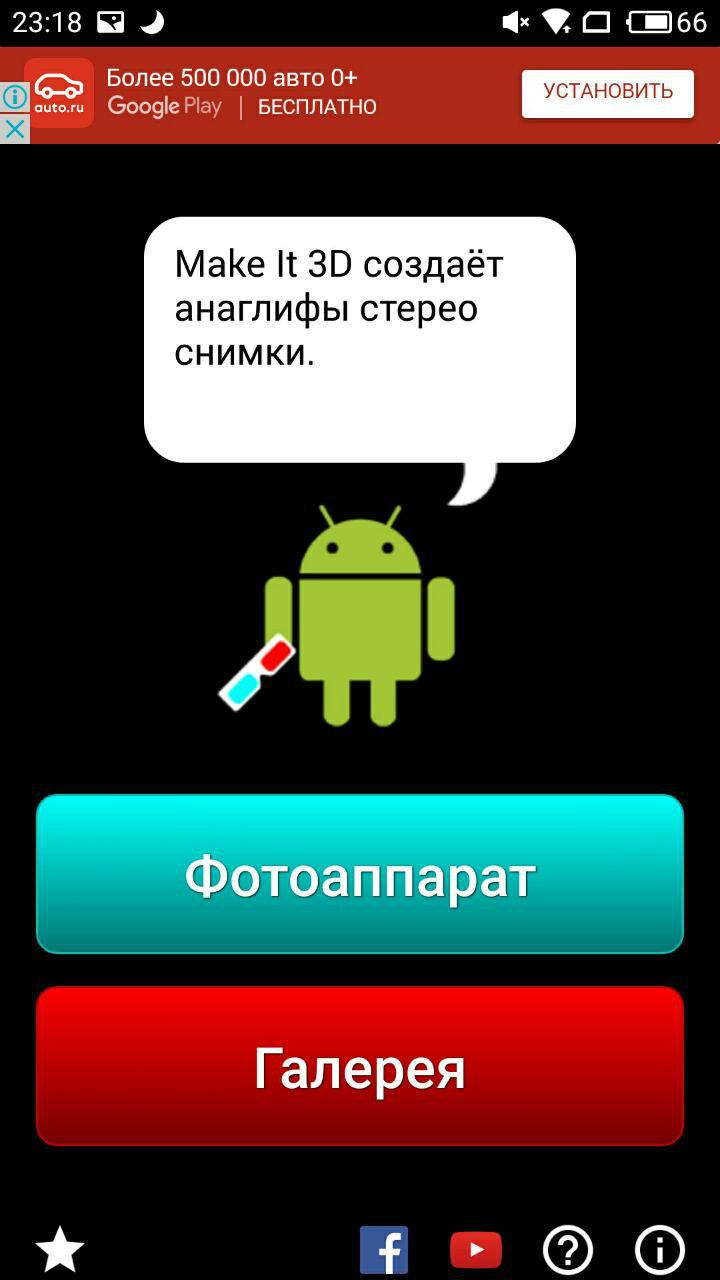
\includegraphics[width=0.45\linewidth]{pics/MakeIt1}
	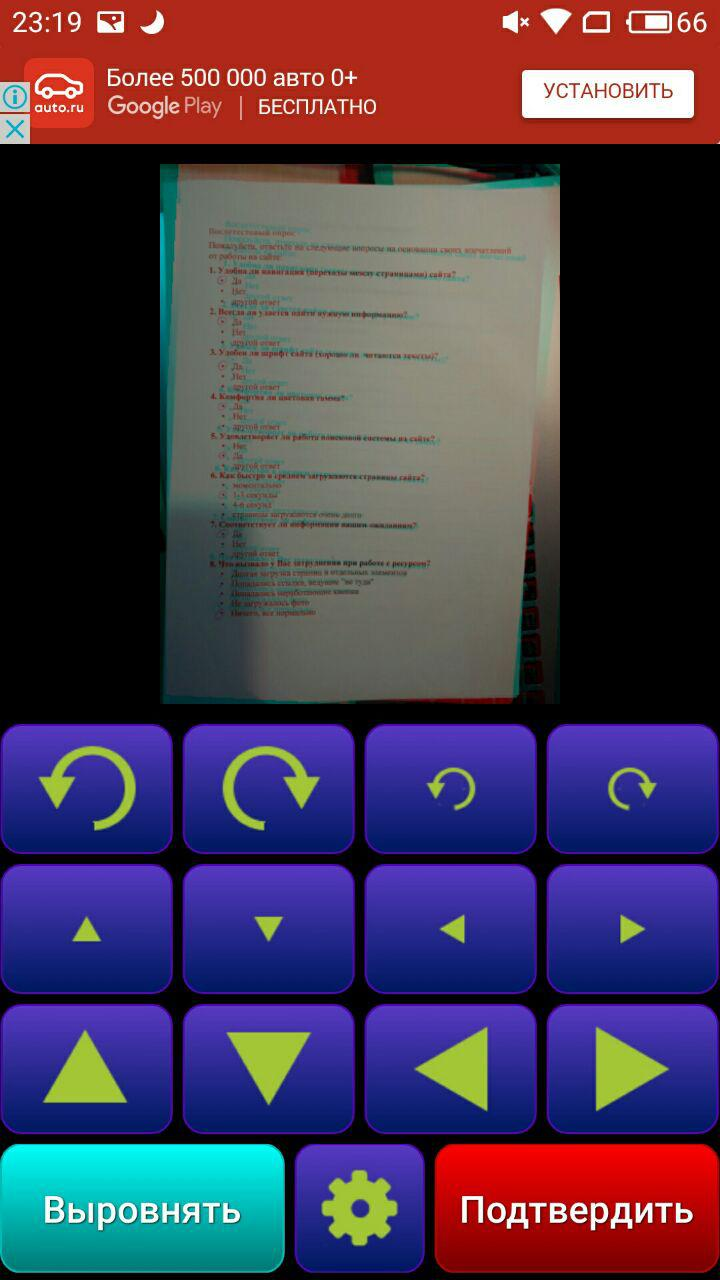
\includegraphics[width=0.45\linewidth]{pics/MakeIt2}
	\caption{MakeIt}
	\label{fig:MakeIt}
\end{figure}

\subsection{3D Effect}

Приложение, создающее анаглиф из одного изображения. Доступна возможность настройки степени смещение и выбор одного из трех вариантов смещения:  по горизонтали, по вертикали, по диагонали. Так предоставлена возможность выбора цвета стереоэффекта, например: красно-голубой, сине-желтый, зелёно-розовый. Изображение сохраняется в фотогалерею смартфона и выводит варианты «шэринга». (рисунок ~\ref{fig:3dEffect})

\begin{figure}[H]
	\centering
	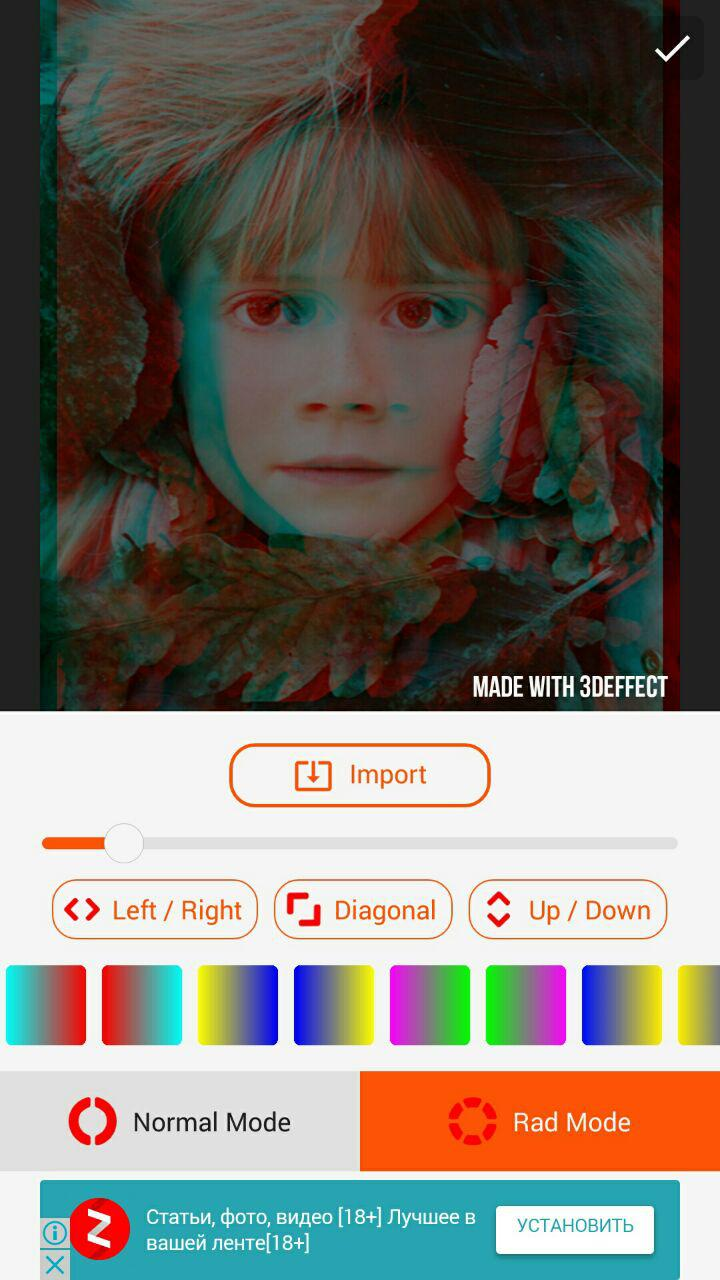
\includegraphics[width=0.45\linewidth]{pics/3dEffect1}
	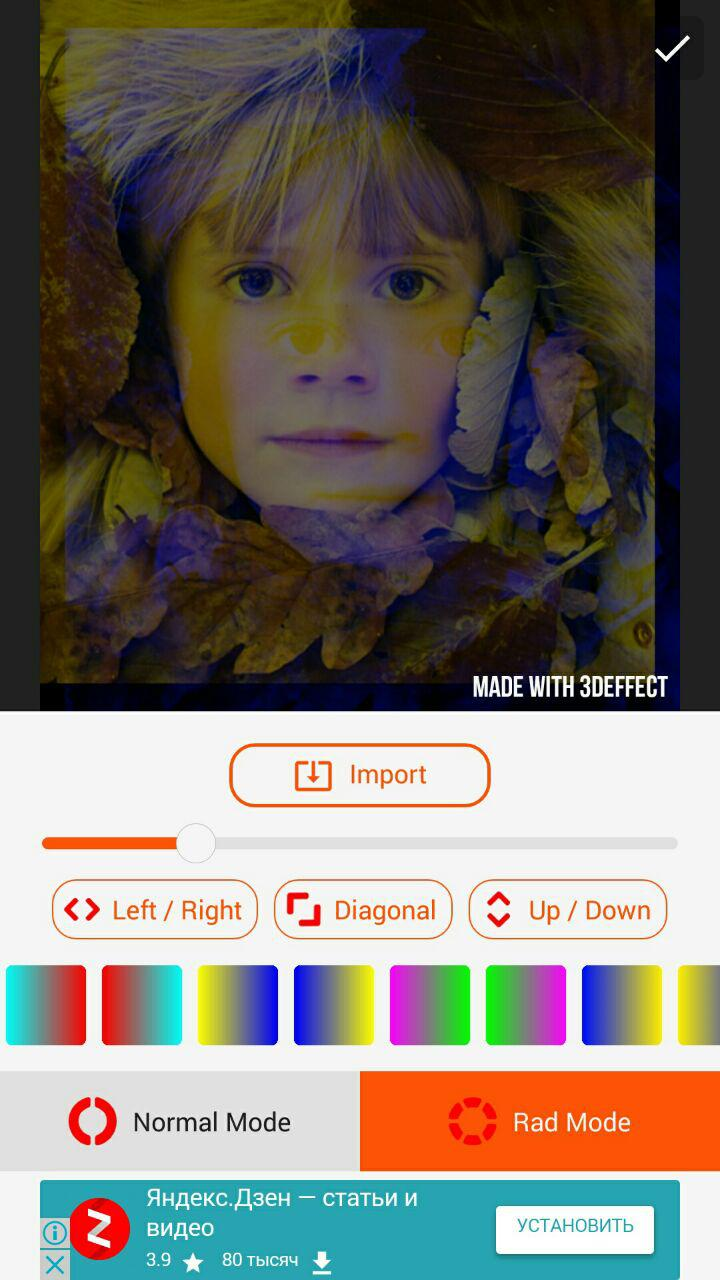
\includegraphics[width=0.45\linewidth]{pics/3dEffect2}
	\caption{3dEffect}
	\label{fig:3dEffect}
\end{figure}

\subsection{Motion Photo}

Инструмент, предоставляемый производителями смартфонов. Впервые появился в iOS 9 в 2015 году под названием Live Photos, а позже аналоги появились в Android-смартфонах, линейке Galaxy от Samsung, начиная с модели S7, а также в Google Pixel 2. Решение в корне отличается от варианта с созданием анаглифа, однако предоставляет возможность оживить фотографию, что так же является и результатом работы нашей разработки. Принцип работы заключается в постоянном сохранении в оперативную память устройства 1-3 секунд изображения с камеры, до момента нажатия на кнопку спуска затвора, после чего сохраняется еще один видеофрагмент. Таким образом, при просмотре обычного фото в галерее смартфона, появляется возможность увидеть живой момент съемки.

\subsection{Fyuse}

Fyuse совмещает в себе возможность создания пространственной фотографии и платформу для общения. По ходу использования приложение фокусируется на объекте, а затем при помощи графических подсказок на экране предлагает обойти объект камерой по орбите. Полученный результат представляет собой снимок, позволяющий перемещать камеру вида по орбите вокруг изображенного предмета при помощи свайпов или гироскопа смартфона. Фотографию можно сохранить или опубликовать прямо во Fyuse, являющейся так же и социальной сетью. (рисунок ~\ref{fig:Fyuse})

\begin{figure}[H]
	\centering
	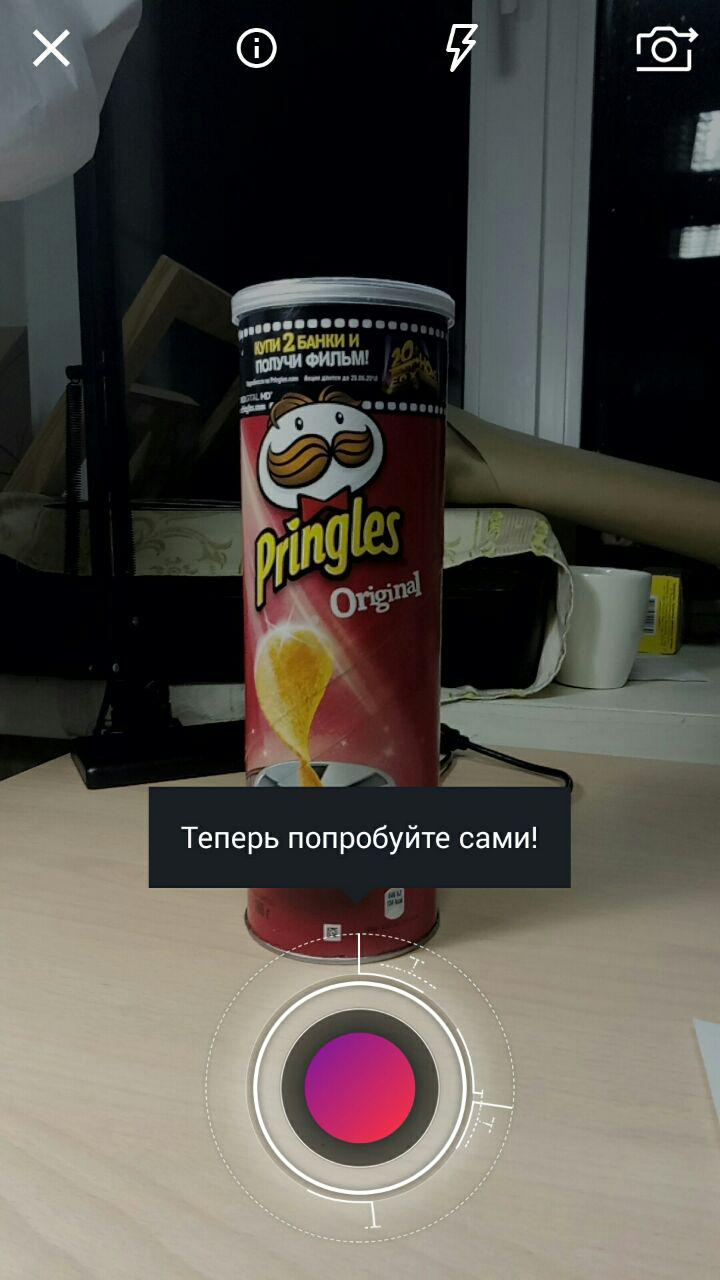
\includegraphics[width=0.45\linewidth]{pics/Fyuse1}
	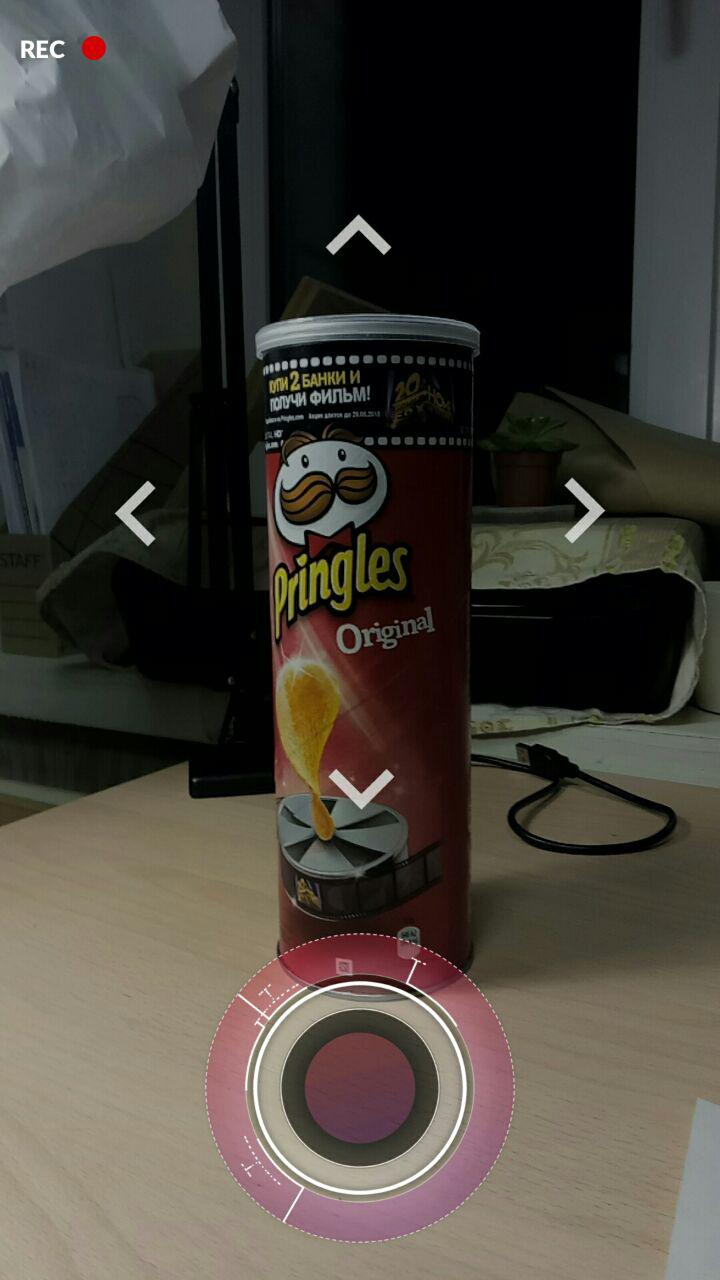
\includegraphics[width=0.45\linewidth]{pics/Fyuse2}
	\caption{Fyuse}
	\label{fig:Fyuse}
\end{figure}

\subsection{Вывод}
По результатам анализа существующих аналогов можно сделать вывод, что разработчики предлагают абсолютно разные способы оживления снимков. Для некоторых требуются определенный манипуляции еще при съемке, некоторые могут работать с готовыми фотографиями. Каждое решение по-своему уникально и интересно. Мы же предлагаем еще одно решение, особенностью которого является «оживление» уже готового снимка.